\section{Evaluation}

\begin{table}[h]
\centering
\caption{Results on \swebenchlite{}. Note: \protect\lock{} indicates approaches that are closed-source (\ie source code is not released).
\protect\cat{} \textbf{indicates approaches built on top of an earlier version of our \tech}.
\textquotesingle-\textquotesingle{} indicates that the relevant information to compute this has not been released. \protect\questionmark{} indicates that multiple models are used, but some of them are not specified. 
\claudesonnet{} is short for \claudesonnet{}onnet.}


\label{tab:main}
\scalebox{0.70}{
\begin{tabular}{ll|rrrrrr}
\toprule
 \multirow{2}*{Tool} & \multirow{2}*{\llm} & \multirow{2}*{\%{} Resolved} & \multirow{2}*{\makecell{Avg.\\{}\$ Cost}} & \multirow{2}*{\makecell{Avg.\\{}\# Tokens}} & \multicolumn{3}{c}{\% Correct Location} \\
 & & & & & Line & Function & File \\
\midrule

\cellcolor[HTML]{e1dcef}\codestoryaide{}~\cite{codestoryaide} \lock{} & \cellcolor[HTML]{e1dcef}\makecell[l]{\openai{} \gptfouro{}+\anthropic{} \claudesonnet} & \cellcolor[HTML]{e1dcef}129 (43.00\%) & \cellcolor[HTML]{e1dcef} - &\cellcolor[HTML]{e1dcef} - &\cellcolor[HTML]{e1dcef}41.7\% &\cellcolor[HTML]{e1dcef}58.7\% &\cellcolor[HTML]{e1dcef}72.0\% \\
\bytedanceagent{}~\cite{marscode} \lock{} & NA & 118 (39.33\%) &  - & - &42.7\% &58.0\% &79.7\% \\
\cellcolor[HTML]{e1dcef}\honeycomb{}~\cite{honeycomb} \lock{} & \cellcolor[HTML]{e1dcef}NA & \cellcolor[HTML]{e1dcef}115 (38.33\%) & \cellcolor[HTML]{e1dcef} - &\cellcolor[HTML]{e1dcef} - &\cellcolor[HTML]{e1dcef}44.3\% &\cellcolor[HTML]{e1dcef}57.0\% &\cellcolor[HTML]{e1dcef}69.3\% \\
\mentatbot{}~\cite{mentatbot} \lock{} & \openai{} \gptfouro{} & 114 (38.00\%) &  - & - &37.3\% &53.3\% &69.3\% \\
\cellcolor[HTML]{e1dcef}\gru{}~\cite{gru} \lock{} & \cellcolor[HTML]{e1dcef}NA & \cellcolor[HTML]{e1dcef}107 (35.67\%) & \cellcolor[HTML]{e1dcef} - &\cellcolor[HTML]{e1dcef} - &\cellcolor[HTML]{e1dcef}38.3\% &\cellcolor[HTML]{e1dcef}54.3\% &\cellcolor[HTML]{e1dcef}75.0\% \\
\isoform{}~\cite{isoform} \lock{} & NA & 105 (35.00\%) &  - & 41,963 &38.7\% &55.3\% &72.0\% \\
\cellcolor[HTML]{e1dcef}\supercoder{}~\cite{supercoder} \lock{} & \cellcolor[HTML]{e1dcef}NA & \cellcolor[HTML]{e1dcef}102 (34.00\%) & \cellcolor[HTML]{e1dcef} - &\cellcolor[HTML]{e1dcef} - &\cellcolor[HTML]{e1dcef}41.7\% &\cellcolor[HTML]{e1dcef}63.7\% &\cellcolor[HTML]{e1dcef}65.7\% \\
\lingma{}~\cite{lingma} \lock{} & \makecell[l]{\openai{} \gptfouro{}+\anthropic{} \claudesonnet} & 99 (33.00\%) &  - & - &40.0\% &58.7\% &75.0\% \\
\cellcolor[HTML]{e1dcef}\factorydroid{}~\cite{factorydroid} \lock{} & \cellcolor[HTML]{e1dcef}NA & \cellcolor[HTML]{e1dcef}94 (31.33\%) & \cellcolor[HTML]{e1dcef} - &\cellcolor[HTML]{e1dcef} - &\cellcolor[HTML]{e1dcef}36.7\% &\cellcolor[HTML]{e1dcef}55.7\% &\cellcolor[HTML]{e1dcef}72.7\% \\
\amazonqagent{}-v2~\cite{amazonqdeveloper} \lock{} & NA & 89 (29.67\%) &  - & - &40.3\% &52.0\% &74.3\% \\
\cellcolor[HTML]{e1dcef}\specrover{}~\cite{specrover} \lock{} & \cellcolor[HTML]{e1dcef}\makecell[l]{\openai{} \gptfouro{}+\anthropic{} \claudesonnet} & \cellcolor[HTML]{e1dcef}93 (31.00\%) & \cellcolor[HTML]{e1dcef}\$0.65 &\cellcolor[HTML]{e1dcef} - &\cellcolor[HTML]{e1dcef} - &\cellcolor[HTML]{e1dcef} - &\cellcolor[HTML]{e1dcef} - \\
\coder{}~\cite{coder} \lock{} & \openai{} \gptfour{} & 85 (28.33\%) & \$3.34 & 323,802 &35.7\% &52.3\% &67.0\% \\
\cellcolor[HTML]{e1dcef}\masai{}~\cite{masai} \lock{} & \cellcolor[HTML]{e1dcef}NA & \cellcolor[HTML]{e1dcef}84 (28.00\%) & \cellcolor[HTML]{e1dcef} - &\cellcolor[HTML]{e1dcef} - &\cellcolor[HTML]{e1dcef}38.7\% &\cellcolor[HTML]{e1dcef}56.3\% &\cellcolor[HTML]{e1dcef}75.0\% \\
\sima{}~\cite{sima} \lock{} & \openai{} \gptfouro{} & 83 (27.67\%) & \$0.82 & - &37.0\% &54.0\% &79.0\% \\
\cellcolor[HTML]{e1dcef}\ibmagent{}~\cite{ibmagent} \lock{} & \cellcolor[HTML]{e1dcef}NA & \cellcolor[HTML]{e1dcef}80 (26.67\%) & \cellcolor[HTML]{e1dcef} - &\cellcolor[HTML]{e1dcef} - &\cellcolor[HTML]{e1dcef}39.7\% &\cellcolor[HTML]{e1dcef}56.7\% &\cellcolor[HTML]{e1dcef}73.3\% \\
\opencsgagent{}~\cite{opencsgstarship} \lock{} & \openai{} \gptfour{} & 71 (23.67\%) &  - & - &39.0\% &61.7\% &90.7\% \\
\cellcolor[HTML]{e1dcef}\amazonqagent{}~\cite{amazonqdeveloper} \lock{} & \cellcolor[HTML]{e1dcef}NA & \cellcolor[HTML]{e1dcef}61 (20.33\%) & \cellcolor[HTML]{e1dcef} - &\cellcolor[HTML]{e1dcef} - &\cellcolor[HTML]{e1dcef}34.0\% &\cellcolor[HTML]{e1dcef}43.7\% &\cellcolor[HTML]{e1dcef}71.7\% \\
\repounderstander{}~\cite{repounderstander} \lock{} & \openai{} \gptfour{} & 64 (21.33\%) &  - & - & - & - & - \\
\midrule
\cellcolor[HTML]{e1dcef}\autocoderover{}-v2~\cite{autocoderovertwo} & \cellcolor[HTML]{e1dcef}\openai{} \gptfouro{} & \cellcolor[HTML]{e1dcef}92 (30.67\%) & \cellcolor[HTML]{e1dcef} - &\cellcolor[HTML]{e1dcef} - &\cellcolor[HTML]{e1dcef}35.0\% &\cellcolor[HTML]{e1dcef}52.3\% &\cellcolor[HTML]{e1dcef}69.3\% \\
\repograph~\cite{repograph} & \openai{} \gptfouro{} & 89 (29.67\%) &  - & - &36.7\% &51.3\% &71.0\% \\
\cellcolor[HTML]{e1dcef}\multirow{1}*{\moatless{}~\cite{moatless}} & \cellcolor[HTML]{e1dcef}\anthropic{} \claudesonnet{} & \cellcolor[HTML]{e1dcef}80 (26.67\%) & \cellcolor[HTML]{e1dcef}\$0.17 &\cellcolor[HTML]{e1dcef} - &\cellcolor[HTML]{e1dcef}38.7\% &\cellcolor[HTML]{e1dcef}54.7\% &\cellcolor[HTML]{e1dcef}78.7\% \\
\cellcolor[HTML]{e1dcef} & \cellcolor[HTML]{e1dcef}\openai{} \gptfouro{} & \cellcolor[HTML]{e1dcef}74 (24.67\%) & \cellcolor[HTML]{e1dcef}\$0.14 &\cellcolor[HTML]{e1dcef} - &\cellcolor[HTML]{e1dcef}36.0\% &\cellcolor[HTML]{e1dcef}52.0\% &\cellcolor[HTML]{e1dcef}73.0\% \\
\opendevincodeact{}~\cite{opendevin} & \anthropic{} \claudesonnet & 80 (26.67\%) & \$1.14 & - &38.0\% &49.7\% &67.3\% \\
\cellcolor[HTML]{e1dcef}\aider{}~\cite{aidar} & \cellcolor[HTML]{e1dcef}\makecell[l]{\openai{} \gptfouro{}+\anthropic{} \claudesonnet} & \cellcolor[HTML]{e1dcef}79 (26.33\%) & \cellcolor[HTML]{e1dcef} - &\cellcolor[HTML]{e1dcef} - &\cellcolor[HTML]{e1dcef}35.3\% &\cellcolor[HTML]{e1dcef}50.0\% &\cellcolor[HTML]{e1dcef}69.7\% \\
\multirow{1}*{\sweagent{}~\cite{sweagent}} & \anthropic{} \claudesonnet{} & 69 (23.00\%) & \$1.62 & 521,208 &40.7\% &54.3\% &72.0\% \\
 & \openai{} \gptfouro{} & 55 (18.33\%) & \$2.53 & 498,346 &29.3\% &42.3\% &58.3\% \\
 & \openai{} \gptfour{} & 54 (18.00\%) & \$2.51 & 245,008 &30.7\% &45.3\% &61.0\% \\
\cellcolor[HTML]{e1dcef}\appmapnavie{}~\cite{appmapnavie} & \cellcolor[HTML]{e1dcef}\openai{} \gptfouro{} & \cellcolor[HTML]{e1dcef}65 (21.67\%) & \cellcolor[HTML]{e1dcef} - &\cellcolor[HTML]{e1dcef} - &\cellcolor[HTML]{e1dcef}29.7\% &\cellcolor[HTML]{e1dcef}44.7\% &\cellcolor[HTML]{e1dcef}59.7\% \\
\autocoderover{}~\cite{autocoderover} & \openai{} \gptfour{} & 57 (19.00\%) & \$0.45 & 38,663 &29.0\% &42.3\% &62.3\% \\
\midrule
\cellcolor[HTML]{e1dcef}\rag{}~\cite{sweagent} & \cellcolor[HTML]{e1dcef}\anthropic{} \claudeopus{} & \cellcolor[HTML]{e1dcef}13 (4.33\%) & \cellcolor[HTML]{e1dcef}\$0.25 &\cellcolor[HTML]{e1dcef} - &\cellcolor[HTML]{e1dcef}22.0\% &\cellcolor[HTML]{e1dcef}30.0\% &\cellcolor[HTML]{e1dcef}57.0\% \\
\cellcolor[HTML]{e1dcef} & \cellcolor[HTML]{e1dcef}\openai{} \gptfour{} & \cellcolor[HTML]{e1dcef}8 (2.67\%) & \cellcolor[HTML]{e1dcef}\$0.13 &\cellcolor[HTML]{e1dcef} - &\cellcolor[HTML]{e1dcef}12.7\% &\cellcolor[HTML]{e1dcef}23.3\% &\cellcolor[HTML]{e1dcef}47.3\% \\
\cellcolor[HTML]{e1dcef} & \cellcolor[HTML]{e1dcef}\anthropic{} \claude{}-2 & \cellcolor[HTML]{e1dcef}9 (3.00\%) & \cellcolor[HTML]{e1dcef} - &\cellcolor[HTML]{e1dcef} - &\cellcolor[HTML]{e1dcef}16.7\% &\cellcolor[HTML]{e1dcef}24.3\% &\cellcolor[HTML]{e1dcef}46.7\% \\
\cellcolor[HTML]{e1dcef} & \cellcolor[HTML]{e1dcef}\openai{} \chatgpt{} & \cellcolor[HTML]{e1dcef}1 (0.33\%) & \cellcolor[HTML]{e1dcef} - &\cellcolor[HTML]{e1dcef} - &\cellcolor[HTML]{e1dcef}6.3\% &\cellcolor[HTML]{e1dcef}11.3\% &\cellcolor[HTML]{e1dcef}27.3\% \\
\midrule
\textbf{\tech{}} & \openai{} \gptfouro{} & 96 (32.00\%) & \$0.70 & 78,166 &35.3\% &52.0\% &69.7\% \\

\bottomrule
\end{tabular}
}
\end{table}

\subsection{Performance on \swebenchlite{}}

Table~\ref{tab:main} shows the main evaluation result of \tech and prior agent-based approaches on \swebenchlite{}. 
We observe that \tech is able to solve \totalsolve out of 300 problems (\totalsolveperc{}).  
While this is not the highest percentage of problems solved on \swebenchlite{}, \tech is extremely competitive compared with prior agent-based approaches while using a much simpler design and overall technique. 
It is important to note here that many of the top techniques are closed-source/commercial and did not release any source code to reproduce experiments or even {trajectories} for further verification. 
\textbf{Compared with all open-source approaches, \tech is able to achieve the highest performance of \totalsolveperc{} (\totalsolve{} / 300) on \swebenchlite.}
Additionally, \tech only costs on average \averagedollarcost{}, which is less than most prior agent-based approaches. 
Comparing against the RAG agentless baselines, we see that while \tech costs slightly more, \tech is also able to fix way more issues.

\begin{wrapfigure}{r}{0.55\textwidth}
  \begin{center}
    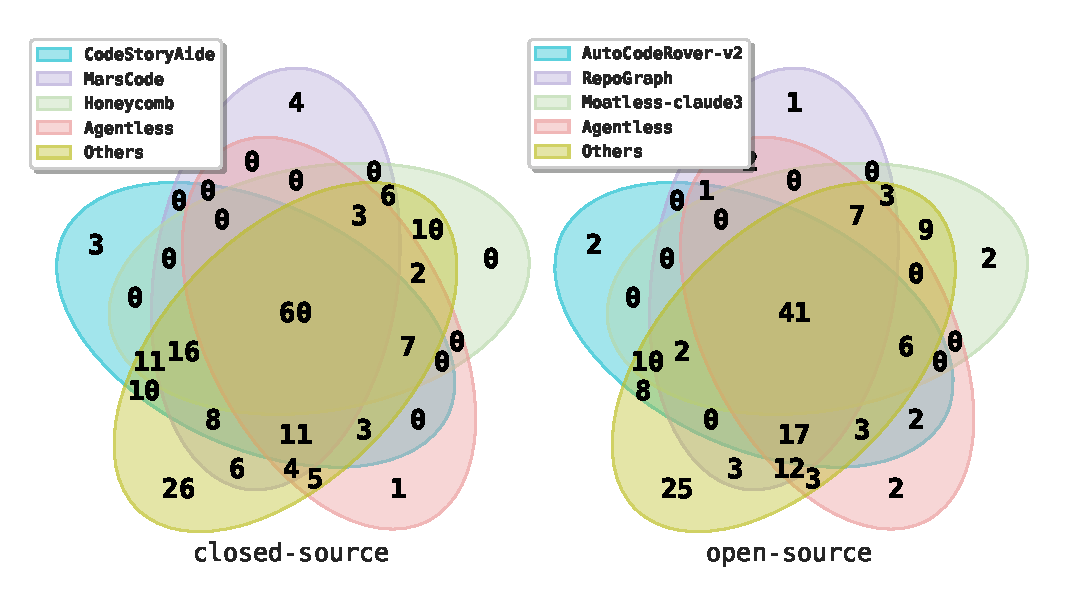
\includegraphics[width=0.55\textwidth]{figs/venn_comparison.pdf}
  \end{center}
  \caption{Venn diagram for issue fixes.}
  \label{fig:venn}
\end{wrapfigure}


\subsubsection{Unique issues fixed.}  Figure~\ref{fig:venn} shows the unique issues solved by \tech compared with the top-performing closed-source / commercial and open-source approaches (``Others'' indicates all other approaches within each category). 
First, we see that compared to the open-source agent-based tools, \tech is able to {fix 2 issues that no other tools can resolve}, showing the success of using a simple agentless approach in solving difficult issues.
Furthermore, even when compared with high-performing commercial approaches, \tech is still able to offer a unique fix. 
This low number of unique fixes can be attributed to the fact there are already tools built on top of earlier versions of \tech (e.g., \isoform{}~\cite{isoform}) or partly inspired by \tech (e.g., \bytedanceagent~\cite{marscode}), thereby reducing the unique issues resolved by \tech.
Nevertheless, our results show that \tech can be competitive/complementary compared to existing agents.

\subsubsection{Localization performance.} In real-world software development, apart from directly fixing the issue, providing the correct edit location to developers is extremely helpful for debugging. 
As such, we examine the locations of the patches generated by each technique compared with the ground truth patch. 
We note here that it is possible to fix a bug in a different location than the ground truth, however comparing against the ground truth patch can still serve as an approximate measure.  
Table~\ref{tab:main} additionally shows the {percentage} of {submitted patches with correct locations} for each tool{, across} line, function, and file levels.
We first observe that the percentage of {patches with correct locations} correlates heavily with the solve rate. 
Interestingly, the highest result for file-level location is \opencsgagent{} at 90.0\%, significantly higher than even the best-performing approaches while at the same time having a relatively low solve rate (23.67\%). 
As \opencsgagent{} is a commercial product that does not provide source code or detailed trajectories, it is difficult to explain this huge difference between localization and repair performance. 
In terms of localization performance, by using our simple hierarchical approach, \tech remains very competitive compared with previous agent-based approaches.

\subsubsection{Reproduction test results.}

\tech uses regression and generated \reproduction tests to perform filtering in order to select the final submission patch. 
Therefore, we evaluate the quality of our generated \reproduction tests. 
We note here that as described in Section~\ref{sec:reproduction_test_generation}, we only use the generated \reproduction test if it can successfully reproduce the original issue in the original repository. 
Out of the 300 problems in \swebenchlite, \tech is able to produce 213 \reproduction tests that output the required reproduction message when evaluated on the original repository.
However, these tests might still be incorrect as a correct \reproduction should also be able to verify that the issue has been correctly resolved.
To evaluate this, we directly apply the ground truth patch provided in \swebench\footnote{Note that the ground truth patch is only applied here to evaluate the test quality, and is not used during the \tech process for selecting the reproduction tests.}.
We found that only 94 tests correctly output the \CodeIn{Issues resolved} message after applying the ground truth patches. 
This steep drop-off can be partially explained as sometimes the issue description provided in the problem may not contain enough information to generate complete test cases for validating a correct solution.
However, this problem is partially mitigated as \tech takes a conservative approach of requiring all patches to pass the regression test suite first and will remove a patch if it cannot pass the regression tests but passes on the generated \reproduction test. 
This reduces the likelihood of an incorrect \reproduction test selecting a correct patch. 
Furthermore, if all generated patches cannot pass the \reproduction test, \tech will fall back on only using the regression test results for selection.
In Section~\ref{sec:test_generation_ablation} we closely examine the impact of using both regression and \reproduction test for patch selection has on the performance.

\begin{wraptable}{r}{0.55\textwidth}
\footnotesize
\centering
\caption{Performance of different localization steps.}
\label{tab:ablationlocation}
\scalebox{0.85}{
\begin{tabular}{l|rrr}
\toprule
Method & Contains GT & LoC & Avg. \$\\
\midrule 

\multicolumn{4}{c}{File level localization} \\ 
\midrule

\cellcolor[HTML]{e1ecff}Prompting-based & \cellcolor[HTML]{e1ecff}78.67\% & \cellcolor[HTML]{e1ecff}3,221 & \cellcolor[HTML]{e1ecff}\$0.02 \\
\makecell[l]{Embedding-based \\ (w/o irrelevant filtering)} & 67.67\% & 3,388 & \$0.05 \\
\cellcolor[HTML]{e1ecff}\makecell[l]{Embedding-based \\ (w/ irrelevant filtering)}& \cellcolor[HTML]{e1ecff}70.33\% & \cellcolor[HTML]{e1ecff}3,622 & \cellcolor[HTML]{e1ecff}\$0.04 \\
\textbf{Combined} & 81.67\% & 3,424 & \$0.06 \\
\midrule
\multicolumn{4}{c}{Related element localization} \\
\midrule
\cellcolor[HTML]{e1ecff}Complete file & \cellcolor[HTML]{e1ecff}53.67\% & \cellcolor[HTML]{e1ecff}778 & \cellcolor[HTML]{e1ecff}\$0.15 \\
\textbf{Skeleton format} & 58.33\% & 698 & \$0.02 \\
\midrule
\multicolumn{4}{c}{Edit location localization} \\
\midrule
\cellcolor[HTML]{e1ecff}Greedy & \cellcolor[HTML]{e1ecff}50.67\% & \cellcolor[HTML]{e1ecff}189 & \cellcolor[HTML]{e1ecff}\$0.06 \\
Direct from file-level & 47.00\% & 208 & \$0.18 \\
\cellcolor[HTML]{e1ecff}Multi-samples merged & \cellcolor[HTML]{e1ecff}56.33\% & \cellcolor[HTML]{e1ecff}342 & \cellcolor[HTML]{e1ecff}\$0.07 \\
\multirow{4}*{\textbf{Multi-samples}} & 49.67\% & 165 & \multirow{4}*{\$0.07} \\
 & 49.33\% & 180 &  \\
 & 49.33\% & 168 &  \\
 & 48.33\% & 213 &  \\

 
\bottomrule
\end{tabular}
}
\end{wraptable}

\subsubsection{Adoption of \tech.} 
Although released very recently, \tech has already received widespread adoption. 
In Table~\ref{tab:main}, there are two baseline tools (indicated via \cat) already built upon earlier versions of our \tech:
\repograph~\cite{repograph} is an open-source tool combining \tech with repository-level graph, while \isoform{}~\cite{isoform} is a closed-source commercial tool also built upon \tech. 
Additionally, \bytedanceagent~\cite{marscode} is partly inspired by \tech in patch sampling/selection and OpenDevin~\cite{opendevin} is in the process of integrating \tech into their ecosystem. 
Furthermore, \tech has also been adopted by OpenAI as the default approach when showcasing the real-world coding performance of GPT-4o on their new \swebenchverified benchmark~\cite{openaiverified}, where \tech also achieves the best performance compared with all other studied agent-based solutions.
At the time of finishing up this draft, OpenAI just released the new o1 model family and also adopted \tech as the top/default approach to showcase their performance on \swebench~\cite{openaioonesystemcard}.%

\subsection{Ablation study on components of \tech} 

Next, we look at how each component in the localization, repair, and patch validation phases contributed to the final \tech performance. 
Unless otherwise specified, we vary the configuration of one component while using the default parameters for all other settings. 

\subsubsection{Localization ablation.}

Table~\ref{tab:ablationlocation} shows the performance and cost for each of the 3 steps in \tech's localization phase.
We show after each localization step the percentage of problems whose ground truth edit locations remain in the location set (``Contains GT''), the average lines of code {of each location set (``LoC'')}, and the average dollar cost of each step (``Avg.\$'').
The \textbf{bold} method indicates the default setting of \tech. 
First, we examine the different configurations of file level localization. 
To start with, for the retrieval method based on embeddings, we see that without including the irrelevant folder filtering to remove irrelevant folders for embedding (described in Section~\ref{sec:localize_suspicious_files}), both the performance and cost become worse. 
This demonstrates the importance of limiting the number of files to consider during embedding and focusing on essential parts of the repository for more cost-efficient and effective localization.
We see that using the prompting-based or the embedding-based retrieval method alone can locate the ground truth file in 78.7\% and 67.7\% of cases respectively. 
This can be further improved by combining them to obtain 81.7\% correct file localization, showing that prompting-based and embedding-based retrieval methods can complement each other in identifying different sets of {relevant} files.


\begin{wraptable}{r}{0.55\textwidth}
\footnotesize
\centering
\caption{Performance of different repair setups.}
\label{tab:ablationrepair}
\scalebox{0.9}{
\begin{tabular}{l|rr}
\toprule
Method & Performance & Avg. \$ \\
\midrule


\cellcolor[HTML]{e1dcef}\makecell[l]{Greedy location\\(40 samples)} & \cellcolor[HTML]{e1dcef}88 (29.33\%) & \cellcolor[HTML]{e1dcef}\$0.22 \\
\makecell[l]{Multi-samples merged \\(40 samples)} & 85 (28.33\%) & \$0.24 \\
\cellcolor[HTML]{e1dcef}\makecell[l]{\textbf{Multi-samples}\\{\textbf{(4 x 10 samples)}}} & \cellcolor[HTML]{e1dcef}96 (32.00\%) & \cellcolor[HTML]{e1dcef}\$0.29 \\

\bottomrule
\end{tabular}
}
\end{wraptable}

Using all of the localized files leads to a large context window ($>$3000).
As such, in our second localization step, we localize to the relevant classes and functions, and are able to drastically reduce the context window ($<$800). 
We compare our input of using skeleton format (described in Section~\ref{sec:localize_related_elements}) to provide a more concise representation with the baseline of using the complete file content.
We observe that by using the complete file content, not only is the cost much higher but also the number of localized groundtruth issues is reduced. 
The reason is most likely that \llm{s} cannot handle long context very well, so providing the entire file contents can confuse the model.
Conversely, by using a more concise representation as the input, we can effectively localize the correct related locations that are needed for inspection and editing. 


Next, \tech localizes to the exact edit locations needed to achieve even more context reduction without losing much of the localization accuracy. 
We compare the different ways we can perform the edit location localization: 1) ``Greedy'': using greedy decoding to obtain one set of edit locations, 2) ``Direct from file-level'': directly go from file-level localization to the edit locations (instead the default of localizing from file-level to related elements and then to edit locations), 3) ``Multi-samples merged'': sample multiple sets of edit locations and merging them into one set, and 4) ``Multi-samples'': sample multiple sets of edit locations. 
We first observe that by directly going from file-level to the edit locations, both the cost and performance are worse. 
The reason is that the model can become confused when providing a large context, demonstrating the importance of our hierarchical localization design.
We also find that when merging multiple samples together, the amount of ground truth localized is higher but at the expense of having to add more context as the input during the repair phase.
Our default settings also sample the edit locations multiple times, however instead of merging, we perform repair on them separately to make use of the fact each sampled location set can provide similar localization performance while also limiting the input context.
In short, by using hierarchical localization steps, \tech can successfully minimize the cost while performing effective localization. 



\subsubsection{Repair ablation.}
We now look at the impact of our different repair setups on the final performance. Table~\ref{tab:ablationrepair} shows the different settings and inputs for our repair phase with their performance and cost.%
Starting with using the greedy location set generated in the edit location generation stage, we observe that we can already achieve very high performance of more than 88 issues fixed.
Similarly, for the ``Multi-samples merged'' where we merged multiple location sets into one, we can also achieve comparable performance.
The performance can be further improved by considering each sampled locations separately (to generate 10 candidate patches each) when performing repair to achieve \totalsolve fixes.
The reason is that each different location sets may localize different ground truth locations and provide different context that can be helpful to fix specific issues.
By using different edit locations and combining with our extensive test filtering and selection stage, \tech can drastically improve the repair performance. 


\begin{wrapfigure}{r}{0.4\textwidth}
  \begin{center}
    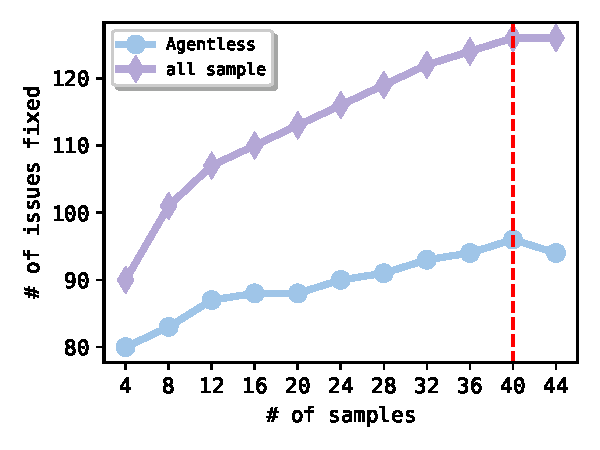
\includegraphics[width=0.4\textwidth]{figs/sample_repair.pdf}
  \end{center}
  \caption{Repair performance as the number of patch samples increases.}
  \label{fig:repair_performance_samples}
\end{wrapfigure}


Next, we examine the impact of using different numbers of sampled candidate patches on the performance of \tech.
Figure~\ref{fig:repair_performance_samples} shows the number of issues fixed as we increase the number of samples. 
Note that the sample interval increases by 4 since we use 4 different sets of locations as input. 
First, we see that by just using 1 greedy sample for each location set, \tech can already achieve a significant number of correct fixes of 80.
We can continue to improve repair performance by adding more samples.
However, we observe that the performance plateaus at around 40 samples where adding additional candidate patches does not improve performance. 
This is because we perform majority voting after test filtering to select the final submission patch, which means that later samples may be ignored since it is difficult for them to offset the majoritively voted patch.  
Interestingly, we can also see from the figure that \emph{if we consider all patch samples (instead of only selecting one patch) for each issue, the total number of possible issues that \tech can solve is 126 (42.0\%).} 
This shows a high upper bound for the potential of \tech with future work being even better patch re-ranking and selection techniques to further improve the overall performance.


\subsubsection{Patch validation ablation.} 
\label{sec:test_generation_ablation}


\begin{wraptable}{r}{0.45\textwidth}
\footnotesize
\centering
\caption{Performance of different patch selection.}
\label{tab:ablationselection}
\scalebox{0.9}{
\begin{tabular}{l|rr}
\toprule
Method & Performance & Avg. \$ \\
\midrule


\cellcolor[HTML]{d9ead3}Majority voting & \cellcolor[HTML]{d9ead3}77 (25.67\%) & \cellcolor[HTML]{d9ead3}\$0.00 \\
+Regression test & 81 (27.00\%) & \$0.01 \\
\cellcolor[HTML]{d9ead3}\textbf{+Reproduction test} & \cellcolor[HTML]{d9ead3}96 (32.00\%) & \cellcolor[HTML]{d9ead3}\$0.25 \\


\bottomrule
\end{tabular}
}
\end{wraptable}

Finally, we examine the impact of our different test generation and patch selection configurations has on performance.
Table~\ref{tab:ablationselection} shows the result and additional cost of different approaches. 
We see that by only using majority voting, we can already achieve 77 correct fixes.
{
By adding the existing regression tests, and filter for candidate patches with the lowest amount of regression errors, we can improve performance to 81 issues resolved.}
Furthermore, the most significant performance improvement was achieved by incorporating additional filtering based on the generated reproduction tests, resulting in the final \tech performance of \totalsolve fixes. 
This demonstrates the impact of our patch selection approach, specifically our \reproduction test generation, which is able to make use of the high number of candidate patches generated and filter for the correct patch for final submission.
However, using \reproduction tests also comes with additional costs as \tech needs to generate these tests which are not provided in the original project repository.

\begin{wrapfigure}{r}{0.4\textwidth}
  \begin{center}
    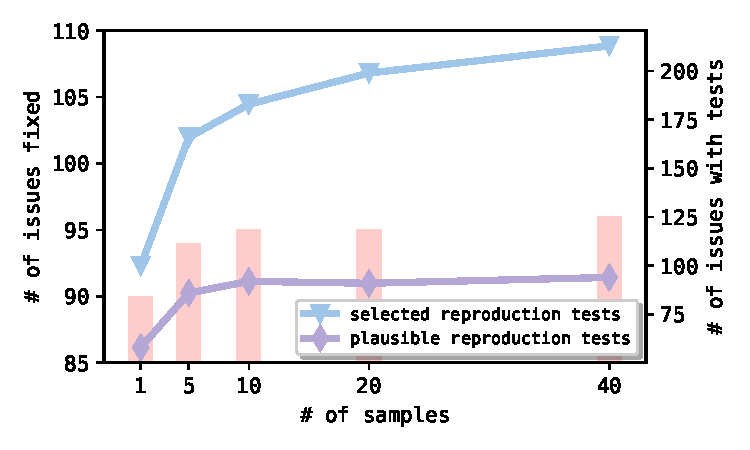
\includegraphics[width=0.4\textwidth]{figs/sample_reproduction.pdf}
  \end{center}
  \caption{Reproduction test and repair results as number of samples increases.}
  \label{fig:reproduction_test_samples}
\end{wrapfigure}



Next, we look at our \reproduction test generation strategy. 
Figure~\ref{fig:reproduction_test_samples} shows the repair performance (bar, left axis), the total number of selected and \plausiblecorrect \reproduction tests (lines, right axis) as we increase the number of candidate \reproduction tests generated per issue. 
Recall that we only select the \reproduction test if it can successfully output the \CodeIn{Issue reproduced} message when evaluated on the original repository.
We further consider a selected \reproduction test as \plausiblecorrect if it can successfully verify that the ground truth developer patch has fixed the original issue (i.e., output \CodeIn{Issue resolved}).
To begin with, when we only generate one \reproduction test (i.e., using the greedy output) per issue, we only produce 100 selected tests for all 300 issues in \swebenchlite with the repair performance being 90. 
We can increase the number of selected \reproduction tests by increasing the number of candidate reproduction tests we generate. 
However, it is interesting to note that the number of \plausiblecorrect \reproduction tests does not increase drastically (apart from going from 1 to 5 samples). 
The reason again is due to some ambiguity in the issue description where it may not contain sufficient information to reproduce and verify the issue has been resolved.
Nevertheless, we observe a small improvement in the number of issues resolved, reaching final performance of 96 correct fixes as we increase the number of candidate \reproduction tests to 40 per issue. 
